\chapter{Эпитаксиальный синтез наногетероструктур}\label{ch:ch1}

\section{Наноструктуры полупроводниковых соединений
A\textsuperscript{III}B\textsuperscript{V}}\label{sec:ch1/sec1}

Полупроводниковые гетероструктуры~--- это искусственные системы, имеющие, по
крайней мере, один гетеропереход~--- границу раздела между двумя веществами с
различными электронными свойствами. Гетероструктуры лежат в основе
полупроводниковых лазеров, светоизлучающих диодов, солнечных элементов,
быстродействующих полевых и биполярных транзисторов, ставших неотъемлемой
частью современных методов передачи информации, электроники, возобновляемой и
ресурсосберегающей энергетики.

Если кристаллические решётки однородных частей (фаз) гетероструктуры взаимно
ориентированы, то гетероструктуру называют эпитаксиальной, а синтез такой
гетероструктуры~--- гетероэпитаксией. Химические элементы гетероструктур
относятся к центральной части периодической таблицы. Элементы III группы могут
вступать во взаимодействие с элементами V группы, при этом образуются, так
называемые, соединения A\textsuperscript{III}B\textsuperscript{V}. Подобным
образом можно получить соединения A\textsuperscript{II}B\textsuperscript{VI} из
элементов II и VI группы (см.~табл.~\cref{tab:tab1}).

Большинство бинарных полупроводниковых соединений служат основой твёрдых
растворов~--- систем соединений переменного состава, в которых атомы различных
элементов расположены в общей кристаллической решётке. Свойства твёрдых
растворов регулируют их составом. Характерный трехкомпонентный твердый раствор
A\textsuperscript{III}B\textsuperscript{V}~--- алюминий\,--\,галлий\,--\,мышьяк
Al\textsubscript{\(x\)}Ga\textsubscript{\(1 - x\)}As, где \(x\)~--- доля узлов
кристаллической решётки III группы, занятых Al, а (\(1 - x\))~--- доля узлов
III группы, занятых Ga. При этом число узлов элементов III и V групп в
кристаллической решётке равно между собой \cite{Kroemer2001}.

\begin{table} [htbp] \centering \begin{threeparttable}% выравнивание подписи по
	границам таблицы \caption{Широко используемые в гетероструктурах химические
	элементы II\,--\,VI групп периодической таблицы}\label{tab:tab1}%
	\begin{tabular}{ p{3cm}  p{3cm}  p{3cm}  p{3cm}  c } \hline \hline II & III &
		IV  & V & VI \\ \hline Be & B  & C  & N   & O   \\ Mg & Al & Si & P   & S
		\\ Zn & Ga & Ge & As  & Se  \\ Cd & In &    & Sb  & Te  \\ Hg &    &    &
	Bi  &   \\ \hline \hline \end{tabular} \end{threeparttable} \end{table}

Важный вклад в становление физики гетероструктур в 60-х годах внесли Жорес
Иванович Алфёров \cite{Alferov2001} и Герберт Крёмер \cite{Kroemer1957}. В 2000
году они получили Нобелевскую премию по физике за разработку полупроводниковых
гетероструктур, используемых в высокочастотной и оптической электронике.

Развитие методов эпитаксиального роста позволяет синтезировать
высококачественные гетероструктуры со сверхтонкими слоями. Уже в 1974 году был
продемонстрирован эффект размерного квантования в полупроводниковых
гетероструктурах AlGaAs/GaAs/AlGaAs с квантовой ямой GaAs \cite{Dingle1974}. Их
спектры поглощения света имели ступенчатый вид с характерной зависимостью от
толщины квантовой ямы.

За последние пятьдесят лет были исследованы различные комбинации материалов,
что позволило разработать приборы с широким набором рабочих характеристик.
Зачастую синтез таких приборных гетероструктур требует нетривиальных
технических решений. Как правило, если материалы с различием параметра
элементарной кристаллической ячейки растут друг на друге, то при увеличении
толщины слоя упругие напряжения релаксируют с образованием дислокаций
несоответствия, которые негативно влияют на электронный транспорт и служат
центрами безызлучательной рекомбинации носителей зарядов
(см.~рис.~\cref{fig:Image_1}). В ряде случаев удается частично решить проблему
согласования решёток синтезом промежуточных периодических метаморфных слоев
\cite{Bolshakov2019}. Тем не менее, выбор комбинаций материалов ростовой
подложки и слоев классических гетероструктур остается ограниченным.

\begin{figure}[ht] \centerfloat{ 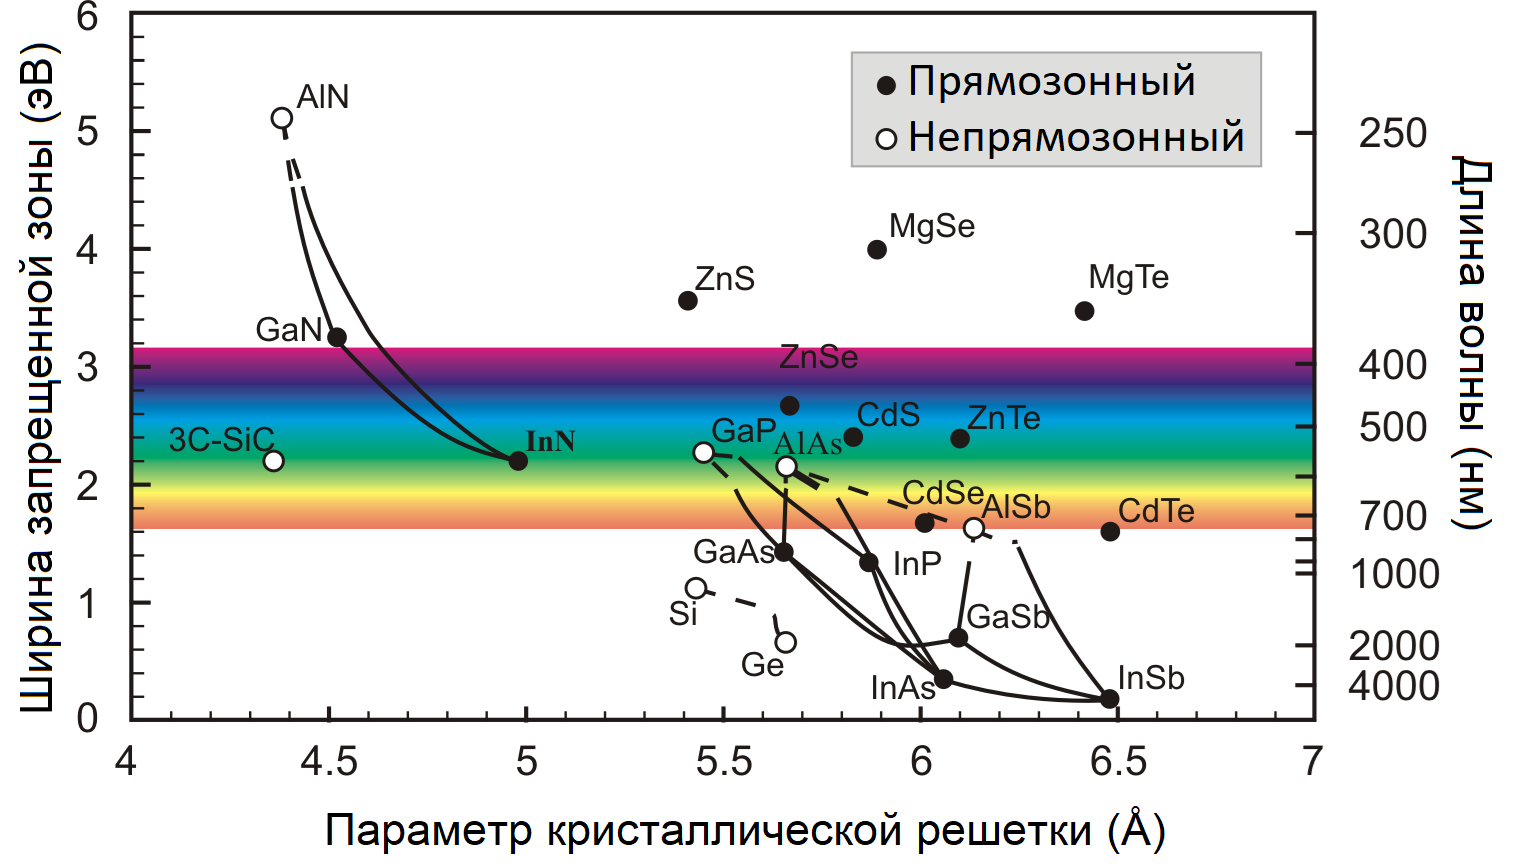
\includegraphics[width=0.9\linewidth]{Image_1}
	} \caption{Связь ширины запрещенной зоны некоторых полупроводников и
параметра кристаллической решётки при 300~\si{\kelvin}}\label{fig:Image_1}
	\end{figure}

Прямозонные A\textsuperscript{III}B\textsuperscript{V} материалы на Si~--- одна
из таких проблемных, но перспективных комбинаций. Развитие технологий
производства полупроводниковых приборов на основе кремния привело к  доминации
этого материала в интегральной электронике и фотовольтаике. При этом он
малопригоден для создания светоизлучающих приборов из-за непрямой зонной
структуры и низкой вероятности излучательных переходов. Развитие технологий
монолитной интеграции оптоэлектронных элементов на Si может снизить стоимость
производства светоизлучающих приборов (за счет отказа от дорогостоящих
A\textsuperscript{III}B\textsuperscript{V} подложек) и заменить электронные
компоненты интегральных схем на оптические (для снижения энергопотребления и
изоляции их компонентов друг от друга).

Монолитная интеграция тонкопленочных структур
A\textsuperscript{III}B\textsuperscript{V} на Si связана с проблемами
несоответствия параметров кристаллических решёток и различием их симметрии:
зарождение A\textsuperscript{III}B\textsuperscript{V} на Si возможно с
различной полярностью, что может приводить к образованию антифазных областей.
Их границы~--- эффективные центры безызлучательной рекомбинации
\cite{Takagi1998}. Образование антифазных областей возможно при росте
материалов с симметрией решётки ниже, чем у подложки. Например, при
формировании соединения с двумя различными атомами в примитивной решётке на
поверхности одноэлементного материала (арсенид галлия (GaAs) на подложке
германия (Ge) или фосфид галлия (GaP) на подложке Si). В случае сингулярной
подложки антифазные области образуются при некогерентном зарождении в плоскости
подложки начиная с разных типов атомов. В случае вицинальной поверхности (когда
нормаль к поверхности подложки не совпадает с основным кристаллографическим
направлением на малый угол, что ведет к образованию ступенчатой поверхности с
террасами основной кристаллографической поверхности) и когерентном зарождении
антифазные границы образуются на ступенях из нечетного количества атомов
(см.~рис.~\cref{fig:Image_2}). В случае когерентного зарождения и ступеней из
четного количества атомов антифазные домены не образуются \cite{Faucher2016}.

\begin{figure}[ht] \centerfloat{ 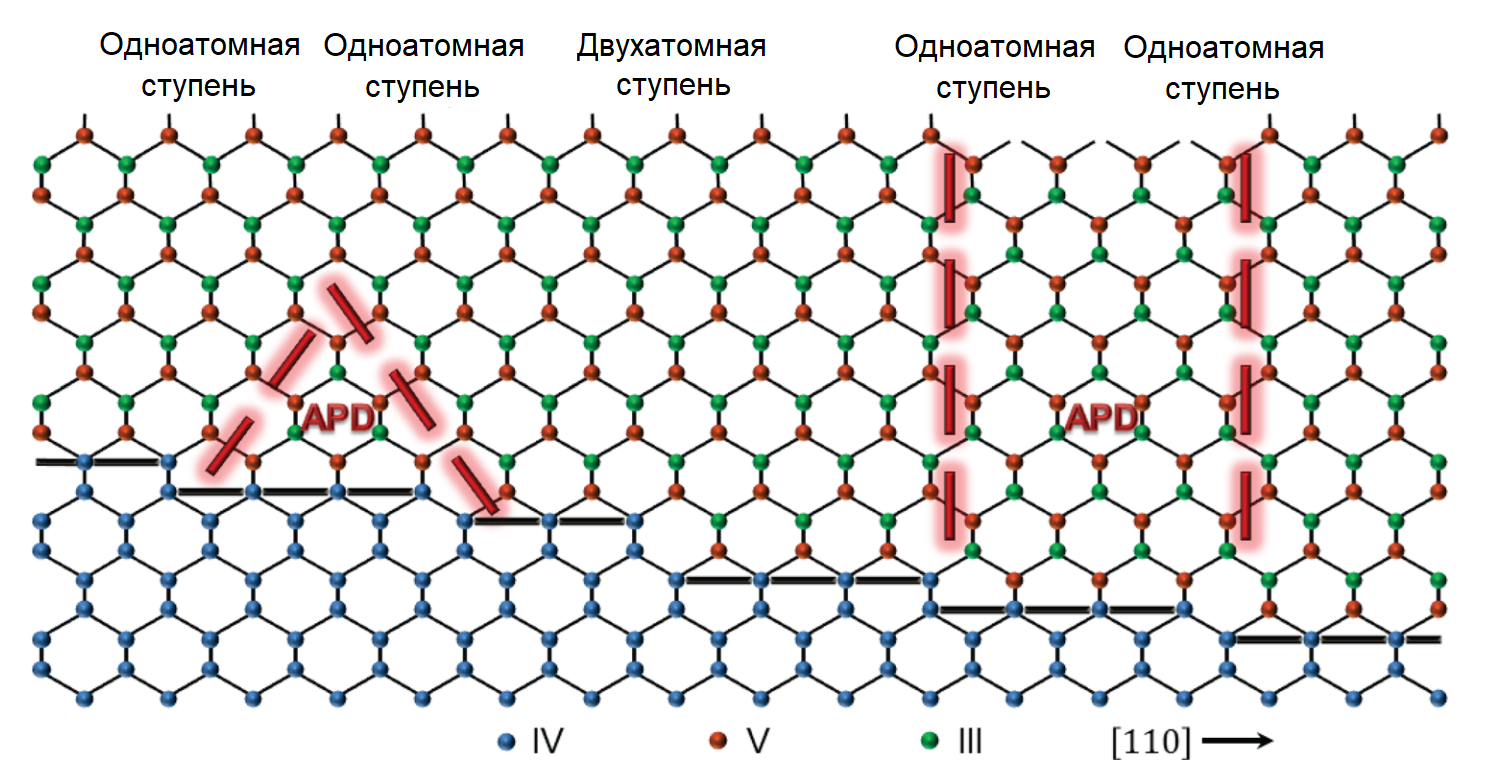
\includegraphics[width=0.9\linewidth]{Image_2}
	} \caption{Схема образования и аннигиляции антифазных доменов на вицинальной
поверхности (001) с моно- и двухатомными ступенями}\label{fig:Image_2}
\end{figure}

Продолжающееся исследования эпитаксиального роста
A\textsuperscript{III}B\textsuperscript{V} слоев на Si (в большей степени это
касается твердых растворов на основе GaP) стимулирует развитие технологий
синтеза функциональных слоев высокого кристаллического качества. Однако, оно
ещё не позволяет достичь достаточно высокого квантового выхода излучения для их
приборного применения.

Альтернативный подход формирования оптоэлектронных элементов на Si включает
синтез A\textsuperscript{III}B\textsuperscript{V} эпитаксиальных наноструктур.
К ним относят квантовые точки, наноостровки, нитевидные нанокристаллы (ННК) и
многообразие гибридных гетероструктур \cite{Tan2018}.

В отличие от послойных гетероструктур, они имеют малую площадь интерфейса с
подложкой и высокое отношение поверхности к объему \cite{Bolshakov2013,
Tchernycheva2007}. Это обеспечивает эффективную релаксацию напряжений и низкую
концентрацию структурных дефектов даже в системах с высоким рассогласованием
кристаллических решёток \cite{Samsonenko2011}.

Более того, наноструктуры предоставляют дополнительные возможности для зонного
проектирования~--- в них удается стабилизировать кристаллическую структуру,
невозможную в объемном материале при нормальных условиях \cite{Mohseni2009}.
Материалы с высокой степенью ионности связи, такие как нитриды, обычно имеют
гексагональную кристаллическую структуру вюрцита (wurtzite, WZ), а материалы с
низкой ионностью, такие как GaP и GaAs,~--- кубическую структуру сфалерита
(zinc-blende, ZB). Однако, при высоком отношении поверхности к объему, в ряде
случаев удается изменять стабильную структуру растущего материала, что
расширяет функциональные возможности гетероструктур \cite{Spirkoska2009}.
Например, GaP с кубической структурой ZB~--- непрямозонный полупроводник, а с
гексагональной структурой WZ~--- прямозонный полупроводник с шириной
запрещенной зоны 2,18--2,25~\si{\electronvolt}, а значит может найти применение
в производстве жёлто-зеленых светодиодов \cite{Assali2013}. Вместе с тем, из-за
симметрии структуре WZ не свойственно двойникование по плоскостям \{111\},
характерное для структуры ZB, что обеспечивает более высокое кристаллическое
совершенство наноструктуры.

Возможность управлять формой наночастиц и их размером в диапазоне от
микрометров до единиц нанометров позволяет формировать структуры с оптическим
или электронным ограничением, что находит применение в оптоэлектронных
приборах. Квантовые точки~--- пример успешного внедрения в промышленность
наноструктур с электронным ограничением. Размер квантовых точек влияет на
расстояние между энергетическими уровнями, а, следовательно, и на спектр
люминесценции. Данный эффект позволяет создавать люминофоры разных цветов из
одного и того же материала. При этом спектр фотолюминесценции имеет узкий и
симметричный пик, а высокое кристаллическое качество обеспечивает высокую
квантовую эффективность.

Для миниатюризации генераторов лазерного излучения требуется уменьшение
оптически активной области резонатора. В множестве работ демонстрируется, что в
ННК может формироваться резонансная стоячая оптическая волна вдоль оси ННК, с
отражением от верхней и нижней граней. Широкий спектральный диапазон генерации
лазерного излучения с оптической и электрической накачкой продемонстрирован на
ННК из ZnO, InGaN, CdSSe, GaAs, InGaAs, AlGaAs, ZnS, CdSe, GaSb, InP и других
материалов \cite{Eaton2016}.

Размер лазеров ограничен дифракционным пределом, который составляет
приблизительно половину длины оптической волны в среде. Уменьшение диаметра ННК
приводит к слабой оптической локализации и снижению добротности резонатора.
Данное ограничение можно обойти, используя ННК в качестве платформы для лазеров
на основе поверхностных плазмон-поляритонов~--- квазичастиц связанного
состояния электромагнитного поля и колебаний электронной плазмы
(см.~рис.~\cref{fig:Image_3}). Коллективные колебания электронов на поверхности
металла имеют значительно меньшую длину волны, чем электромагнитные волны той
же энергии, что позволяет уменьшить размер активной области лазера
\cite{Oulton2009}.

\begin{figure}[ht] \centerfloat{ 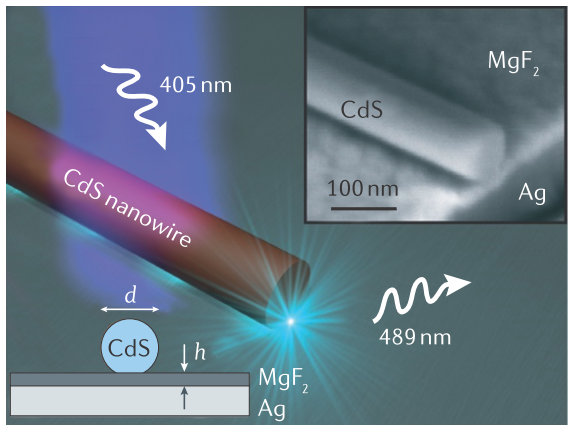
\includegraphics[width=0.6\linewidth]{Image_3}
	} \caption{Изображение ННК CdS на серебряной подложке, образующие резонатор
лазера на основе поверхностных плазмон-поляритонов при оптическом возбуждении
\cite{Oulton2009}}\label{fig:Image_3} \end{figure}

В общем случае форма, размер и поверхностная плотность наноструктур влияет на
их взаимодействие со светом и определяет эффективность вывода или захвата
излучения. Этот эффект находит применение в просветляющих покрытиях солнечных
элементов \cite{Mozharov2015b, Krogman2005} и определяет диаграмму
направленности светоизлучающих приборов на основе массивов наногетероструктур
\cite{Eaton2016}.

Несмотря на достигнутые результаты, остаются не до конца изучены закономерности
формирования самоорганизованных наноструктур, устанавливающие взаимосвязь
морфологии, кристаллической структуры и оптических свойств с ростовыми
условиями и предварительной подготовкой подложки. Изучение данных
закономерностей позволит развить методы синтеза самоорганизованных наноструктур
для применения в приборах оптоэлектроники.

\section{Механизмы формирования эпитаксиальных наноструктур на
кремнии}\label{sec:ch1/sec2}

\subsection{Подготовка кремниевых подложек к росту}\label{subsec:ch1/sec2/sub1}

В результате изготовления, транспортировки и хранения на поверхности Si
подложек остаются загрязнения, а естественный поверхностный оксида имеет
неоднородную толщину и требует высоких температур отжига для сгона. Для
воспроизводимости эксперимента поверхность Si подложки должна быть чистой и
атомарно гладкой, поверхностный оксид иметь контролируемую толщину. Поэтому для
синтеза полупроводниковых структур требуется специальная подготовка Si подложек
перед ростом.

В данной работе использовался один из распространенных методов подготовки~---
метод Шираки \cite{Ishizaka2019}. Он подразумевает кипячения в органических
растворителях и аммиачно-перекисном растворе (для очистки от загрязнений),
несколько циклов попеременной обработки в азотной (для окисления поверхности) и
плавиковой кислотах (для травления поверхностного оксида), завершая
формированием единиц монослоев нестехиометрического поверхностного оксида в
перекисно-кислотном растворе, аммиачно-перекисном растворе или азотной кислоте.
Подготовленные подложки сразу же загружают в эпитаксиальную установку.

Сформированный поверхностный оксид защищает поверхность Si от загрязнения и,
как правило, подлежит удалению отжигом в эпитаксиальной установке, но в
некоторых случаях оксид может играть роль модификатора ростовой поверхности,
так как влияет на поверхностную энергию и смачиваемость поверхности металлом
III группы. Металлический Ga при нанесении на поверхность оксида формируется в
виде массива капель, которые протравливают тонкий слой оксида в местах
поверхностных дефектов. Такие капли могут служить катализатором для
самокаталитического роста ННК GaAs и GaP по механизму
пар\,--\,жидкость\,--\,кристалл (ПЖК).

\subsection{Механизм роста пар\,--\,жидкость\,--\,кристалл
(ПЖК)}\label{subsec:ch1/sec2/sub2}

Впервые механизм ПЖК описан Вагнером и Эллисом в 1964 году на примере роста Si
ННК на подложке Si(111) методом газофазной эпитаксии
(см.~рис.~\cref{fig:Image_4}) \cite{Wagner1964}. Авторы напыляли на подложку
тонкий слой золота (Au), который отжигали при 950~\si{\degreeCelsius} в
реакторе. При этом Si из подложки смешивался с Au с образованием жидких капель
Au:Si. Сплав Au:Si с атомной долей Si 18,6\,\% имеет точку эвтектики при
363~\si{\degreeCelsius}, поэтому может быть жидким при температурах значительно
ниже точки плавления компонентов (Si: 1414~\si{\degreeCelsius}, Au:
1064~\si{\degreeCelsius}).

\begin{figure}[ht] \centerfloat{ \subcaptionbox{\label{fig:Image_4_1}}{%
			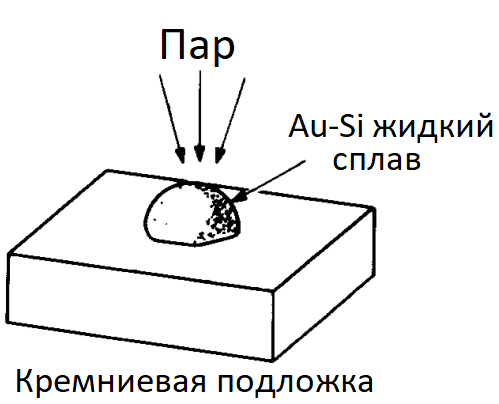
\includegraphics[width=0.3\linewidth]{Image_4_1}}
			\subcaptionbox{\label{fig:Image_4_2}}{%
		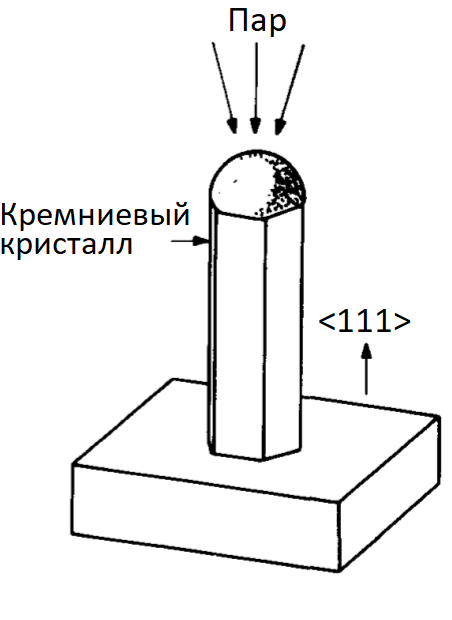
\includegraphics[width=0.3\linewidth]{Image_4_2}} } \legend{Начальные
	условия: жидкая Au капля катализатора на подложке~(а), рост ННК с каплей
катализатора на вершине~(б)} \caption{Схема синтеза Si ННК по механизму ПЖК
\cite{Wagner1964}}\label{fig:Image_4} \end{figure}

Под воздействием газообразного SiCl\textsubscript{4} капля Au перенасыщается
атомами Si. Реакция разложения при низкой температуре катализируется Au каплей,
поэтому её называют катализатором. Эта терминология сохраняется и в случае
молекулярно-пучковой эпитаксии (МПЭ), когда не происходит химического катализа,
а компоненты поставляются на подложку в виде одноэлементных молекул. В таком
случае капля выполняет роль резервуара материала, в котором скорость
конденсация выше, чем скорость образования и роста зародышей по механизму
пар\,--\,кристалл.

Поддерживаемое перенасыщение в капле вызывает непрерывное осаждение Si на
границе жидкость\,--\,кристалл, что приводит к удлинению ННК. Диаметр ННК
определяется размером капли.

Au также используют для роста A\textsuperscript{III}B\textsuperscript{V} ННК,
однако оно легко диффундирует внутрь ННК с образованием локализованных
энергетических уровней, что приводит к деградации времён жизни носителей заряда
\cite{Breuer2011}. Чтобы избежать включений инородного материала существует
альтернативный вариант~--- использовать в качестве катализатора собственный
металл III группы. В таком случае в капле катализатора III группы  с
перенасыщением растворяются только элементы V группы \cite{Breuer2011,
Bolshakov2017}, что ограничивает возможность независимого управления осевой и
радиальной скоростью роста \cite{Dubrovskii2015, Dubrovskii2012a}.
Зародышеобразование и морфология самокаталитических ННК очень чувствительны к
отношению потоков V/III: капля не образуются, если оно слишком велико, а вместо
этого растут островки по механизму пар\,--\,кристалл. В обратной ситуации в
капле накапливается металл III группы с её закономерным увеличением.

Рост ННК под каплей происходит послойно, на что указывают ростовые эксперименты
на установках, совмещенных с просвечивающим электронным микроскопом (ПЭМ)
\cite{Hofmann2008, Wen2009, Jacobsson2016}. При смене подаваемого материала с
сохранением капли могут формироваться аксиальные гетероструктуры. Параллельно
осевому росту идут процессы без участия капли по механизму пар\,--\,кристалл:
радиальной рост ННК и формирование массива паразитных островков. В случае
полного потребления капли катализатора механизм пар\,--\,кристалл становится
доминирующим, что позволяет формировать гетероструктуры типа
ядро\,--\,оболочка.

\subsection{Кристаллическая структура и политипизм соединений
A\textsuperscript{III}B\textsuperscript{V}}\label{subsec:ch1/sec2/sub3}

Политипизм~--- разновидность полиморфизма, при которой в разных кристаллических
модификациях элемента или химического соединения можно выделить периодичные в
двух направлениях слои с идентичным (или почти идентичным) строением.
Обладающие политипизмом вещества называются политипами. Для существования
политипов необходимо, чтобы принципиально одинаковый способ наложения слоёв
(смещение, вращение) мог дать как минимум два неэквивалентных расположения
второго слоя относительно первого. В плоскости плотноупакованного слоя политипы
имеют одинаковый параметр решётки, в перпендикулярном направлении периоды
различны и кратны расстоянию между соседними осями.

Система Л.\,С.~Рамсделла наиболее компактна для обозначения политипов, хотя и
неоднозначна для политипов с одинаковым числом слоёв в элементарной ячейке при
разных последовательностях укладки. В ней цифрой указывается число слоёв в
одной элементарной ячейке, а буквой C, H, R или T обозначается симметрия
решётки (C~--- кубическая, H~--- гексагональная, R~--- ромбоэдрическая и T~---
тригональная). Соединения A\textsuperscript{III}B\textsuperscript{V} образуют
два политипа: ZB~(3C) и WZ~(2H) (см.~рис.~\cref{fig:Image_5}).

\begin{figure}[ht] \centerfloat{ \hfill \subcaptionbox{\label{fig:Image_5_1}}{%
			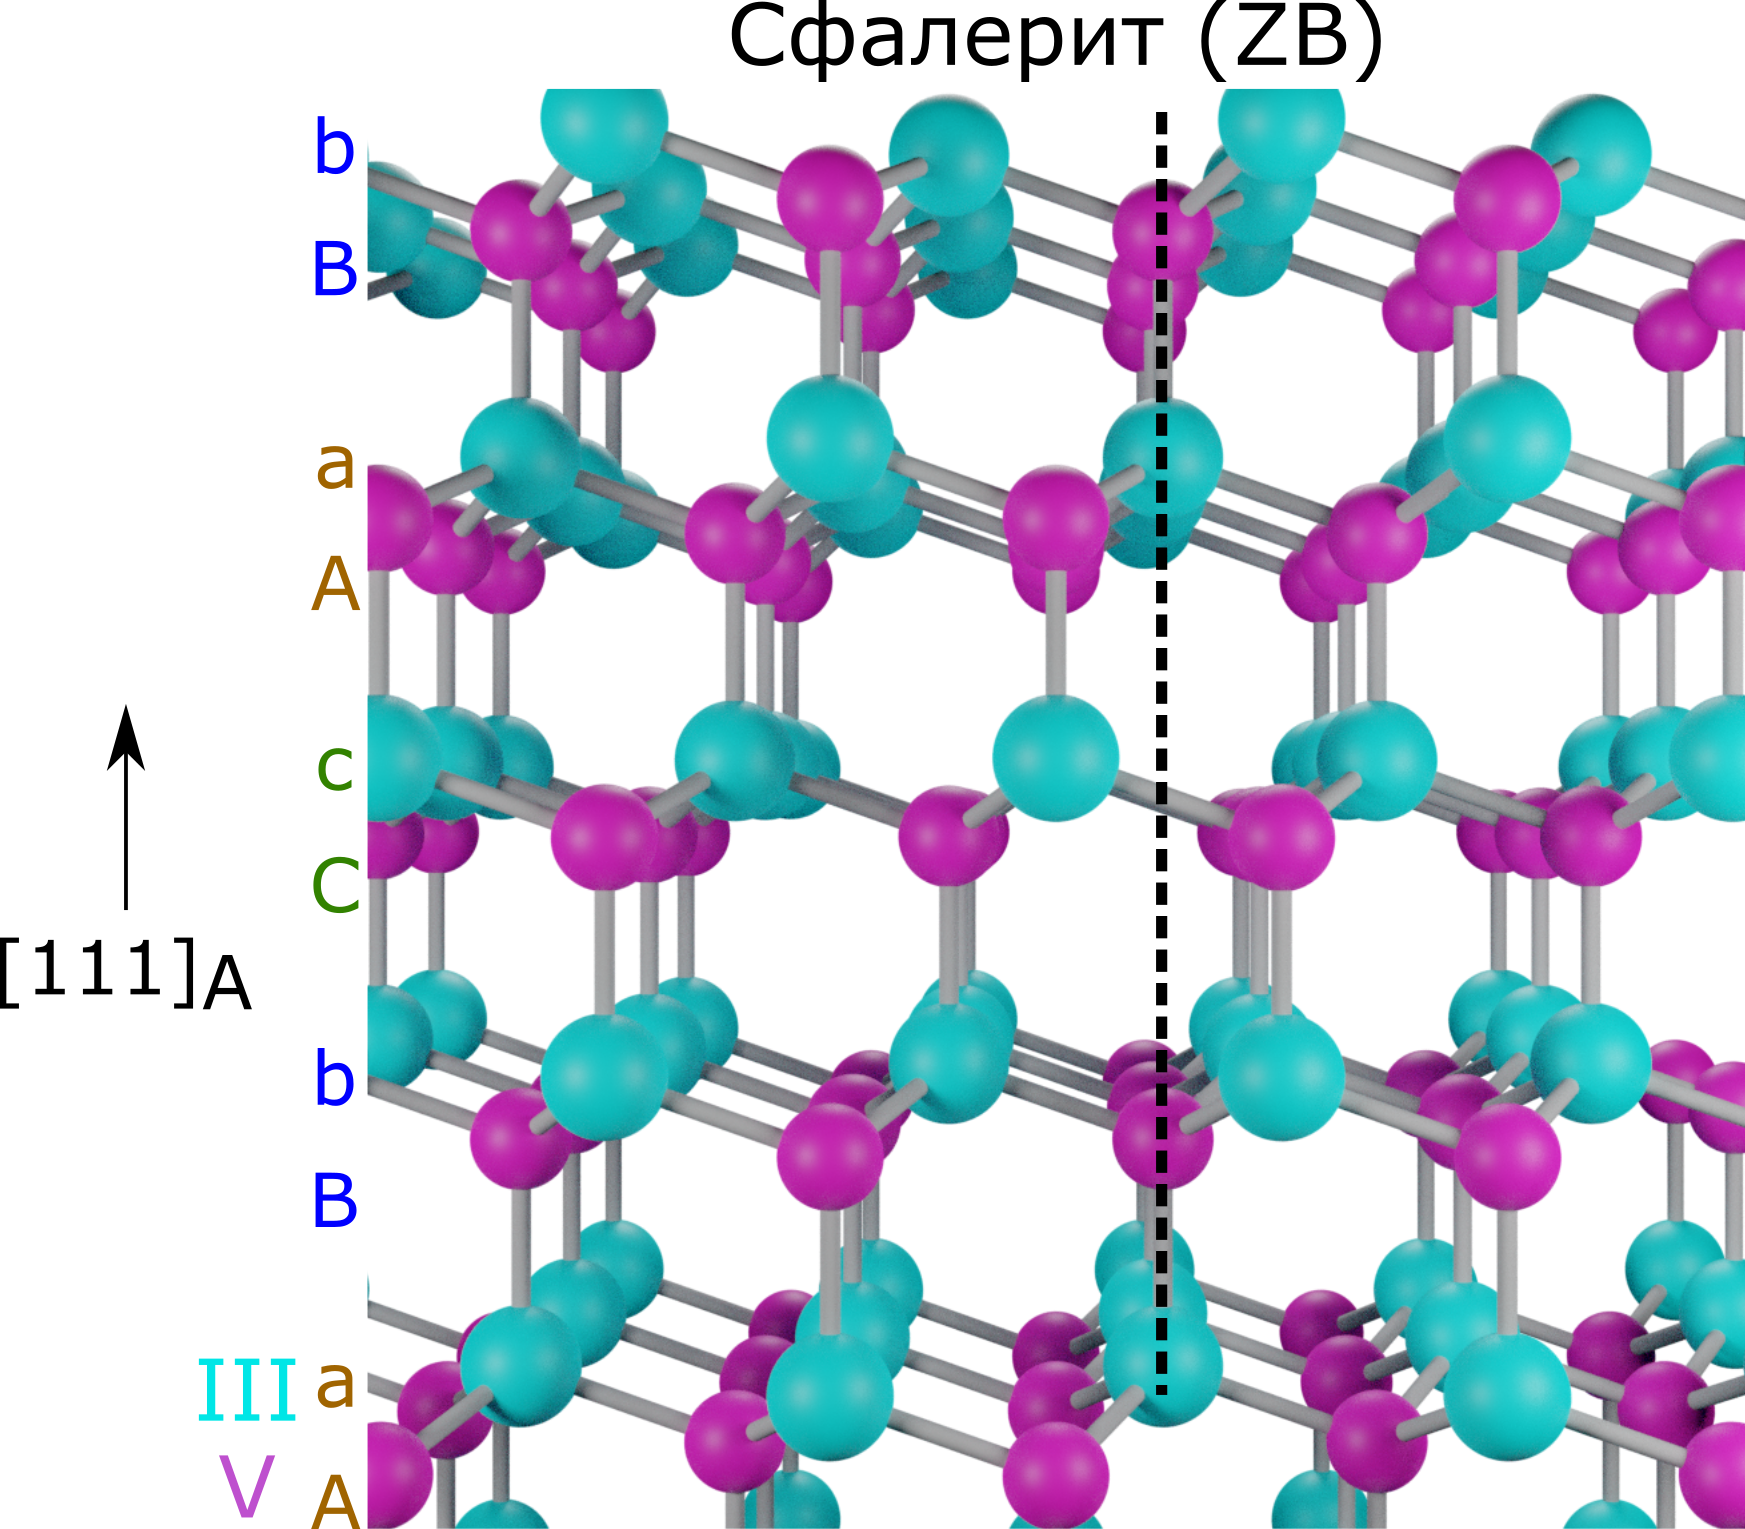
\includegraphics[width=0.3\linewidth]{Image_5_1}} \hfill
			\subcaptionbox{\label{fig:Image_5_2}}{%
		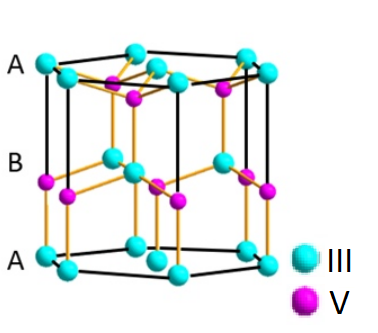
\includegraphics[width=0.35\linewidth]{Image_5_2}} \hfill }
		\caption{Кристаллическая структура ZB\,(3C)~(а) и
		WZ\,(2H)~(б)}\label{fig:Image_5} \end{figure}

Кристаллическая структура ZB схожа с кристаллической структурой Si (структурой
алмаза), которую можно представить как две кубических гранецентрированных
решётки, смещенных друг относительно друга по главной диагонали куба на
четверть её длины.

В случае решёток типа ZB\,(3C) и WZ\,(2H) поверхности (111) и
\((\overline{1}\overline{1}\overline{1})\) неэквивалентны (в случае WZ говорят
о плоскостях (0001) и \((000\overline{1})\)). Структуру ZB\,(3C) можно
представить в виде каркаса тетраэдров AB\textsubscript{4} или
BA\textsubscript{4}. Все тетраэдры ориентированны одинаково, что фактически
приводит к симметрии тетраэдра, а не куба. Каждая вершина тетраэдра общая для
трех соседних тетраэдров. Направление связи между ближайшими атомами А (группы
III) и В (группы V) в кристаллической решётке ZB обозначается <111>. В
структуре алмаза, в элементарной ячейке которой атомы только одного элемента,
эти тетраэдры эквивалентны между собой. На поверхности (111) атом А связан с
тремя атомами В нижележащего монослоя или атом B связан с одним атомом A
нижележащего монослоя. На поверхности
\((\overline{1}\overline{1}\overline{1})\) ситуация обратная: атом B связан с
тремя атомами A нижележащего монослоя или атом A связан с одним атомом B
нижележащего монослоя. Плоскость (111) называют А-полярной, а противоположную
ей~--- В-полярной. A- и B-полярные плоскости также обозначают (111)A и (111)B
соответственно.

Можно определить поверхность (111)A, как оканчивающуюся элементами III группы,
а поверхность (111)B, как оканчивающуюся элементами V группы, однако в условиях
эпитаксиального роста терминация поверхности определяется ростовыми условиями.

Подобным же образом структуру WZ\,(2H) можно представить в виде каркаса
тетраэдров AB\textsubscript{4} или BA\textsubscript{4}. Структура WZ отличаются
от ZB лишь взаимной ориентацией тетраэдров. Периодичность вдоль направления
<111> типа ABCABC\dots, где каждая из букв A, B и C обозначает латеральную
ориентацию слоя толщиной в два атома, состоящего из одного слоя с атомами
группой III и одного слоя с атомами группы V, соответствует структуре ZB
(см.~рис.~\cref{fig:Image_5}). Периодичность вдоль направления <0001> типа
ABAB\dots соответствует структуре WZ \cite{Kriegner2011}. Аналогично плоскости
(0001) и \((000\overline{1})\) обозначают как (0001)A и (0001)B.

\subsection{Эпитаксиальная ориентация
A\textsuperscript{III}B\textsuperscript{V} наноструктур на
Si}\label{subsec:ch1/sec2/sub4}

Эпитаксиальная ориентация наноструктур может быть наглядно продемонстрирована
на примере ННК. Как правило, наноструктуры растут вдоль кристаллографического
направления, которое минимизирует полную свободную энергию \cite{Wagner1964}.
Полная свободная энергия равна сумме объемного вклада, энергии границ раздела
катализатор\,--\,пар, катализатор\,--\,кристалл и пар\,--\,кристалл. Последние
два вклада зависят от кристаллической ориентации границы раздела. При
образовании первого монослоя по механизму ПЖК доминирует вклад энергией границы
раздела катализатор\,--\,кристалл.

ННК преимущественно растут ортогонально поверхности с самой низкой
поверхностной свободной энергией \cite{Wagner1964}. У материалов
A\textsuperscript{III}B\textsuperscript{V} с кристаллической решёткой ZB самую
низкую поверхностную свободную энергию имеет грань (111)B, а у материалов
A\textsuperscript{III}B\textsuperscript{V} со структурой WZ~--- грань (0001)
\cite{Fortuna2010}. Поэтому ННК растут преимущественно вдоль направлений <111>B
и <0001> соответственно. Ориентация ННК относительно поверхности Si подложки в
зависимости от её кристаллографической ориентации для двух возможных случаев
ориентации ZB зародышей показана на рисунке \cref{fig:Image_6}.

\begin{figure}[ht] \centerfloat{ \subcaptionbox{\label{fig:Image_6_1}}{%
		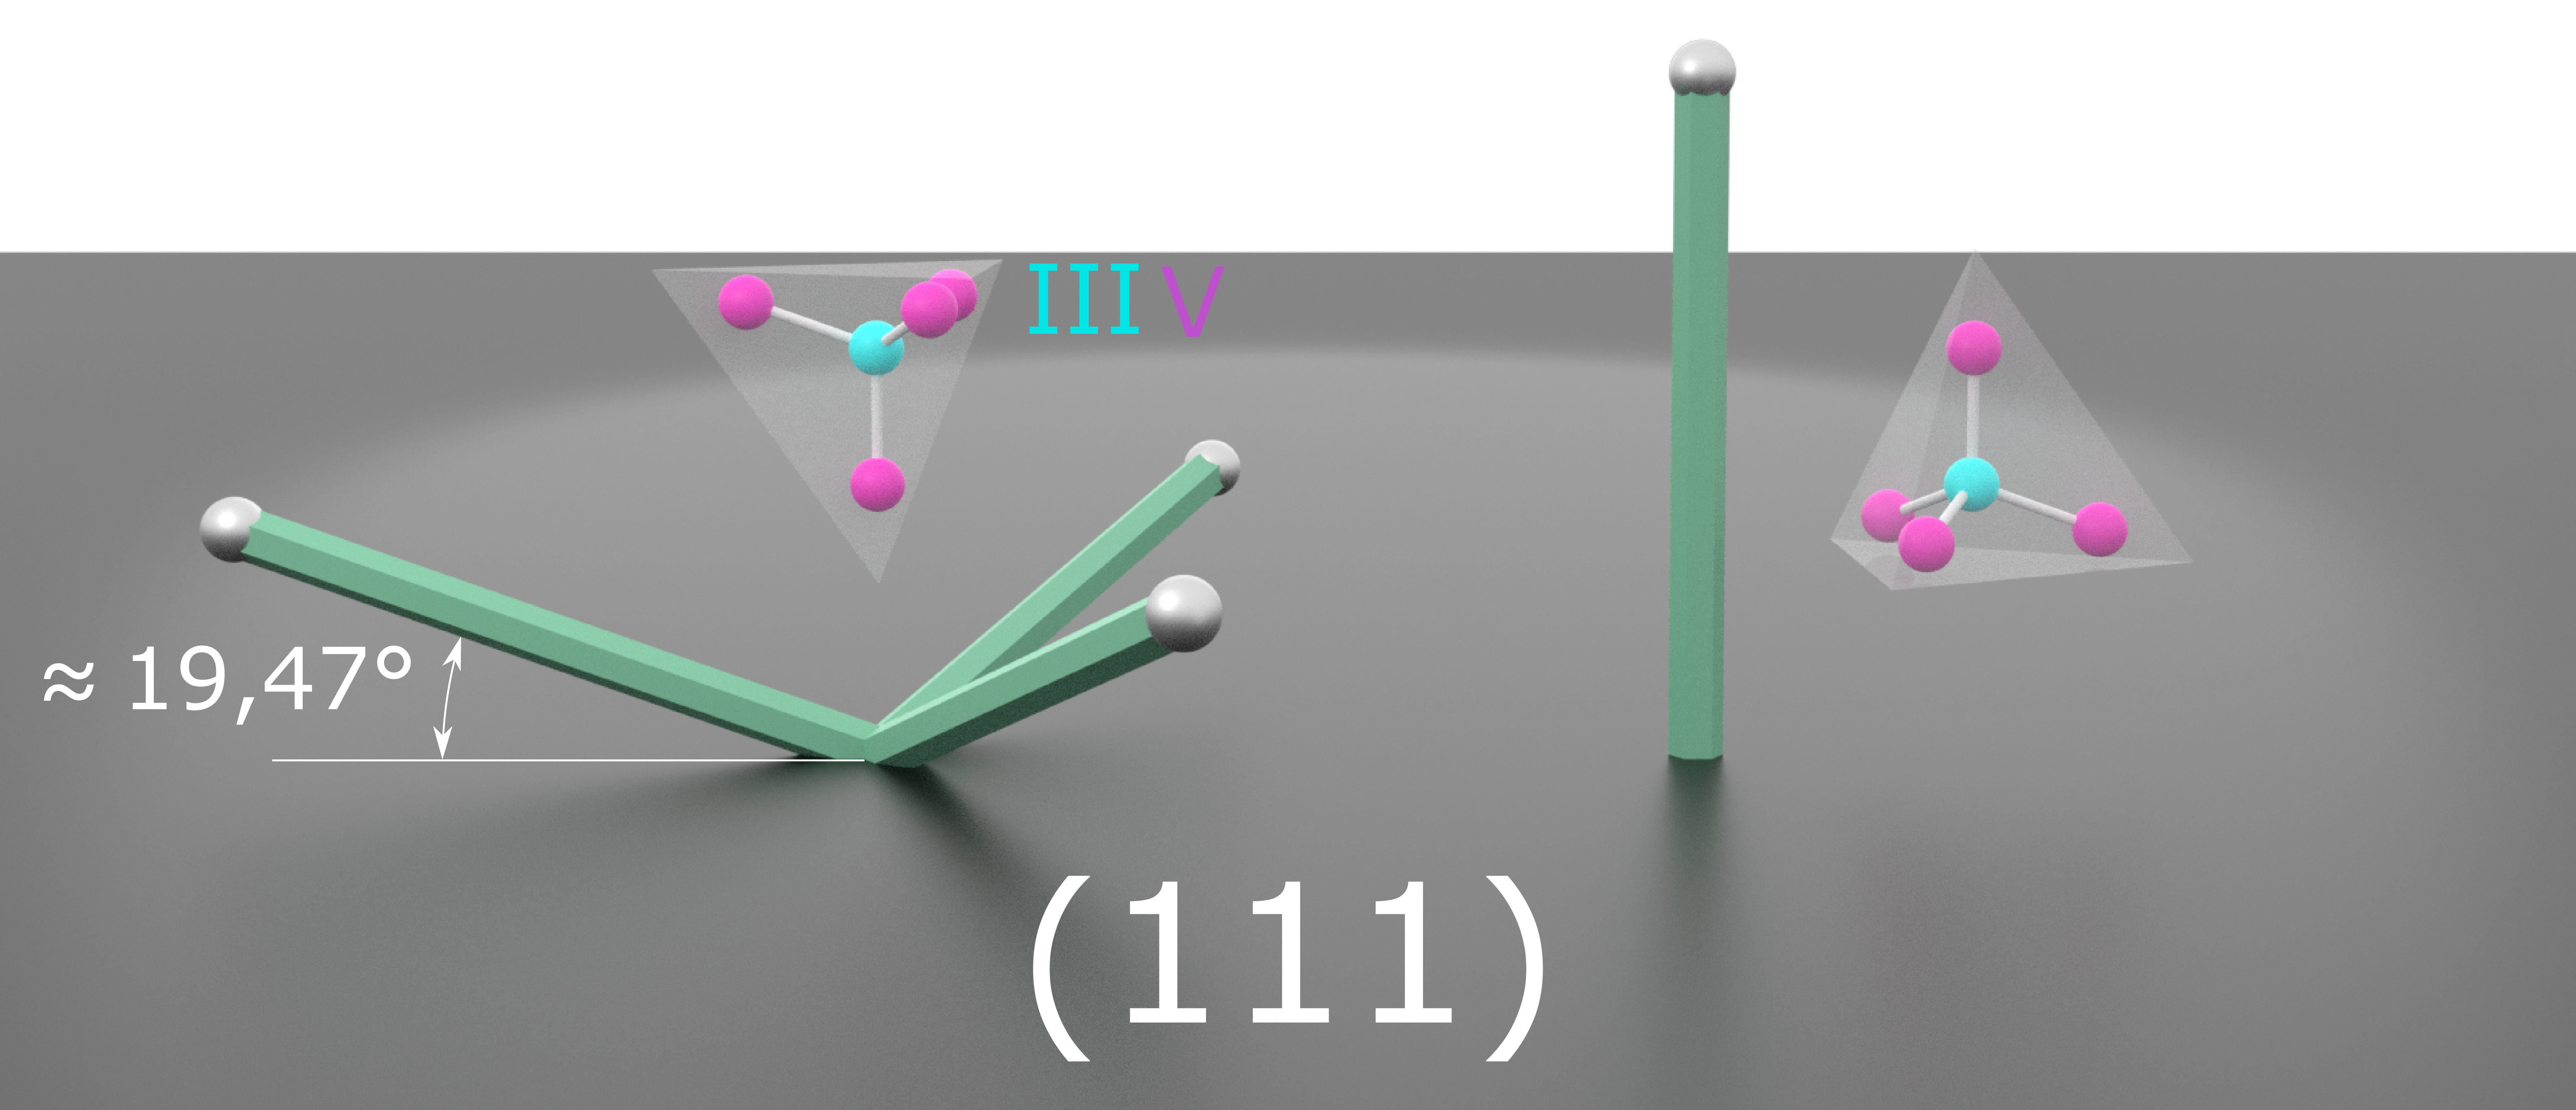
\includegraphics[width=0.9\linewidth]{Image_6_1}}

		\subcaptionbox{\label{fig:Image_6_2}}{%
			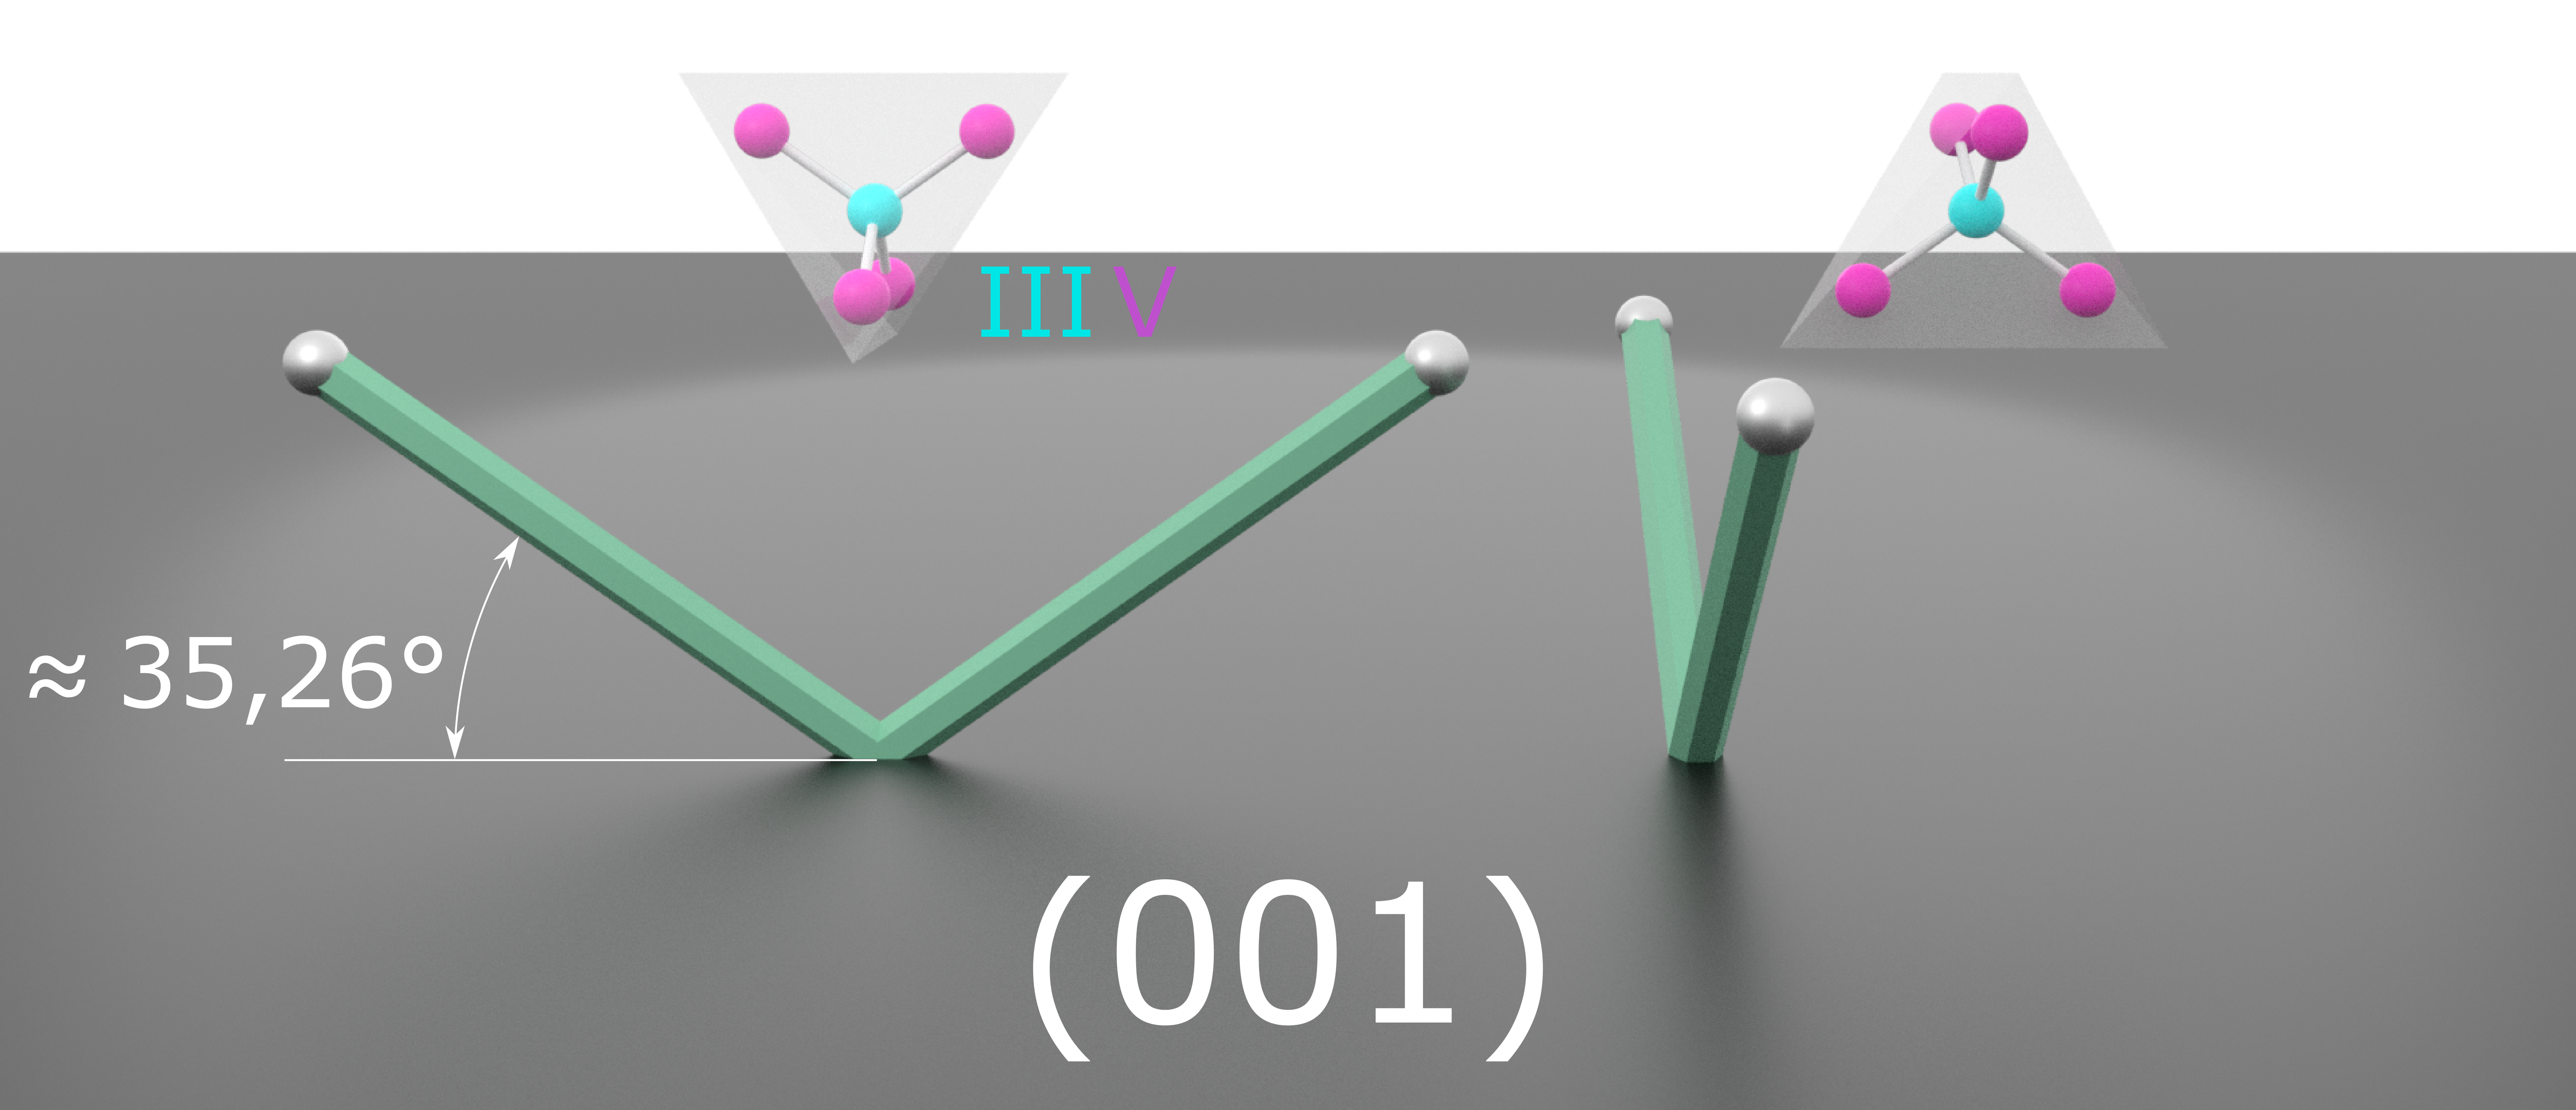
\includegraphics[width=0.44\linewidth]{Image_6_2}}
			\subcaptionbox{\label{fig:Image_6_3}}{%
		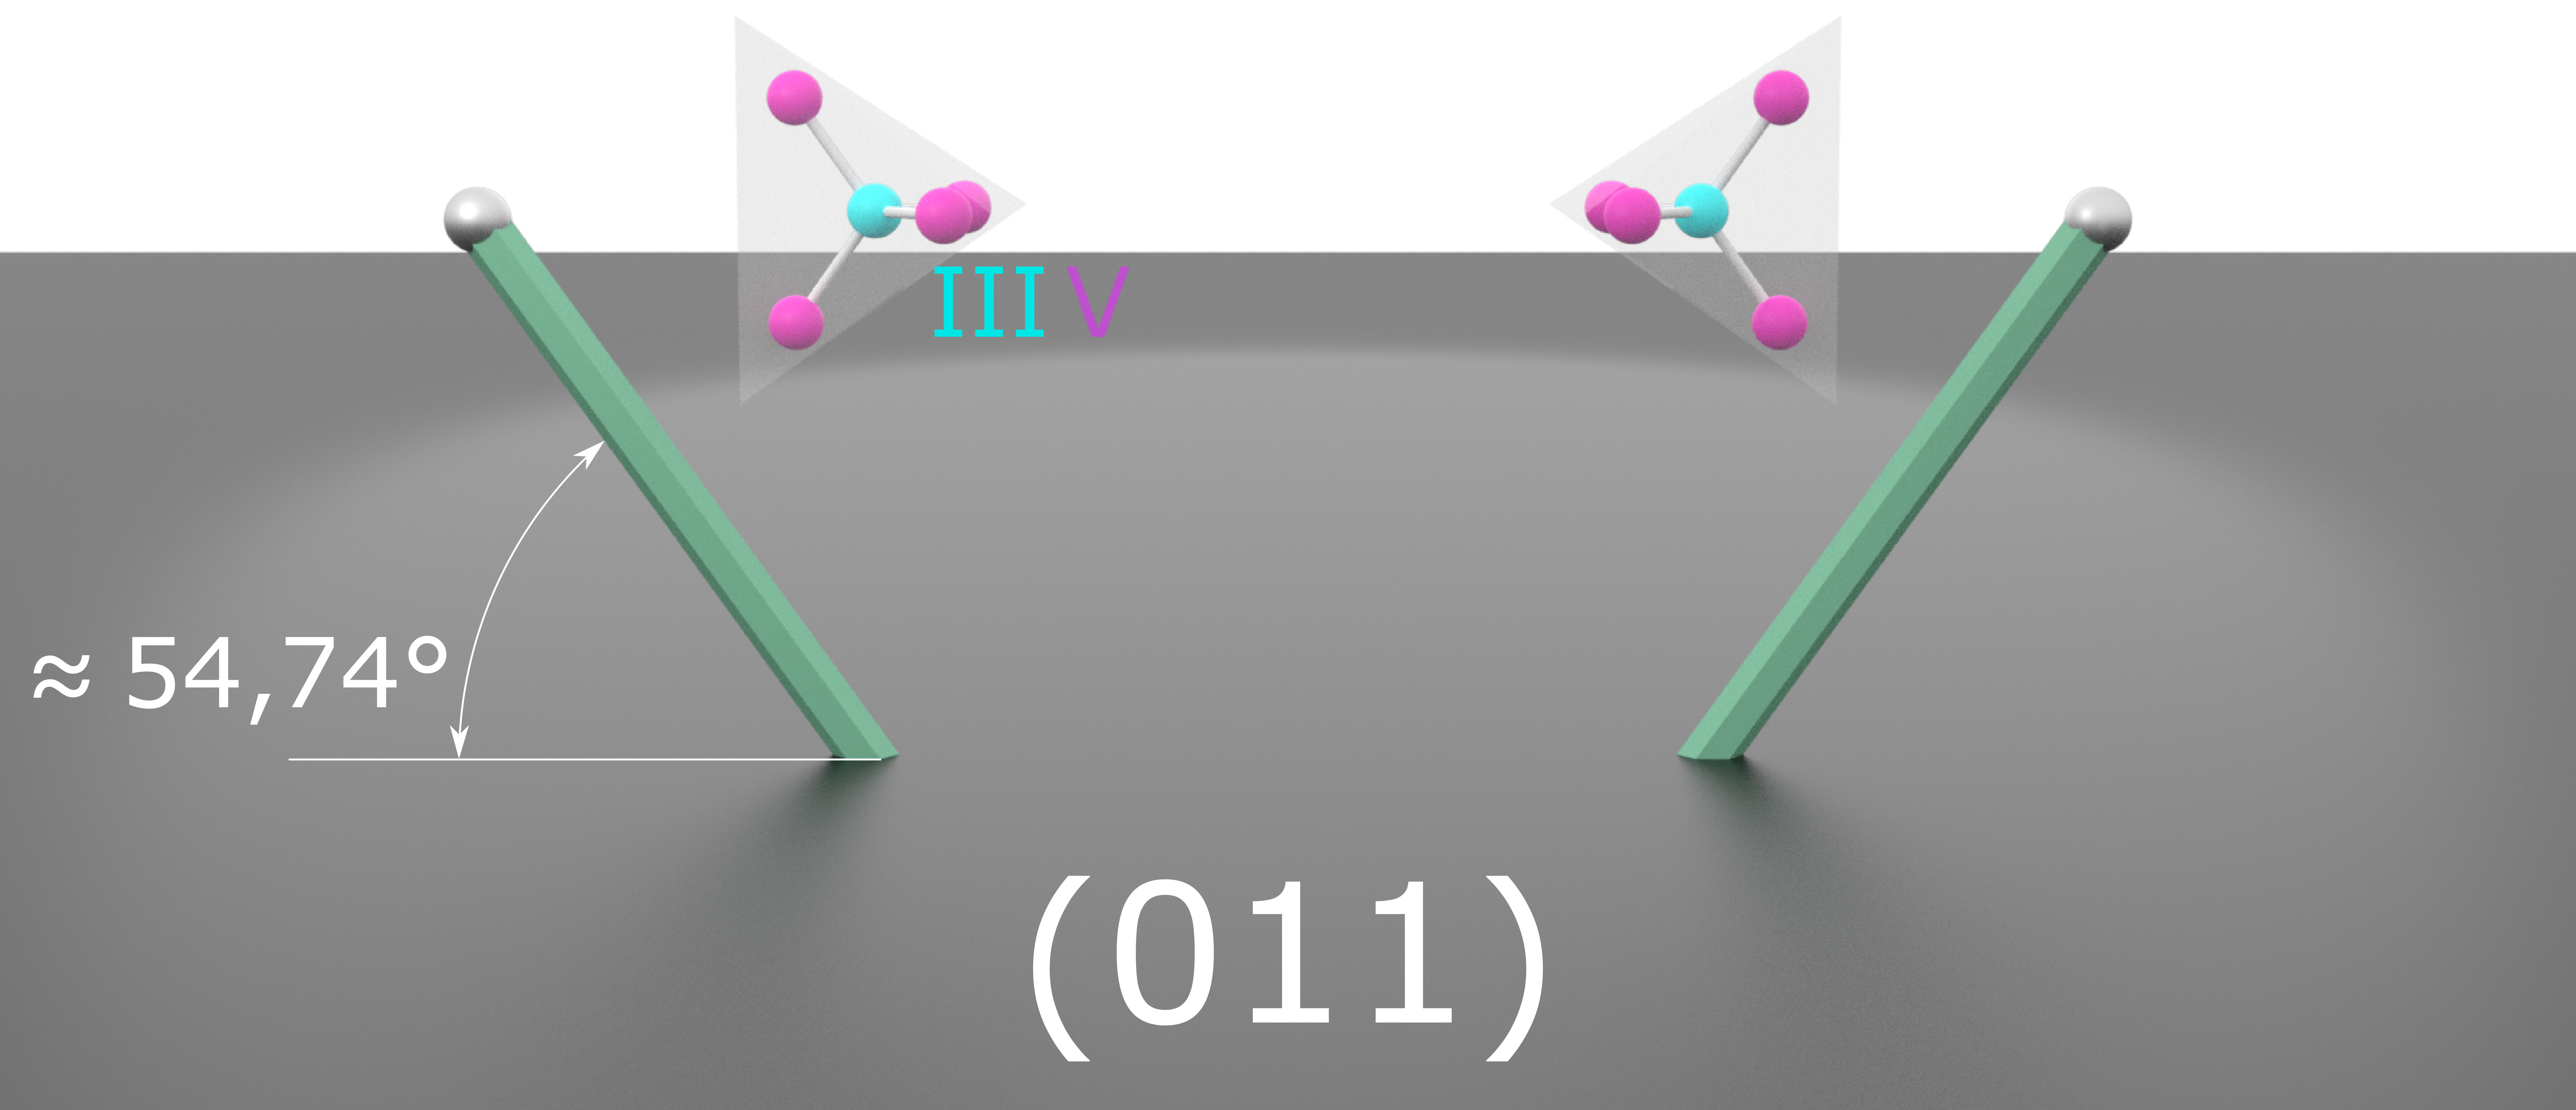
\includegraphics[width=0.44\linewidth]{Image_6_3}} } \legend{Ориентации
	подложек: (111)~(а), (001)~(б) и (110)~(в)} \caption{Схематическое
изображение направлений роста <111>B и эпитаксиальных ориентаций ННК
относительно поверхности подложек Si различной кристаллографической
ориентации}\label{fig:Image_6} \end{figure}

Так как A\textsuperscript{III}B\textsuperscript{V} ННК растут вдоль направления
<111>B, то в случае образования на подложках Si(111) зародыша с ориентацией
B~--- ННК растут вертикально, а в случае образования зародыша с ориентацией
A~--- под углом к подложке в трёх эквивалентных направлениях <111>B
(см.~рис.~\cref{fig:Image_6_1}). Если ZB зародыш с ориентацией A испытывает
вращательное двойникование вокруг оси <111>, ортогональной поверхности
подложки, то ННК растут вдоль трёх дополнительных направлений, развернутых на
180\textdegree вокруг данной оси.

\subsection{Двумерные дефекты и формирование WZ/ZB перехода в
A\textsuperscript{III}B\textsuperscript{V}
наночастицах}\label{subsec:ch1/sec2/sub5}

В процессе роста A\textsuperscript{III}B\textsuperscript{V} наночастиц
образуются следующие типы двумерных дефектов:  для ZB структуры типичны дефекты
вращательного двойникования на 180\textdegree вокруг осей <111> (начало и конец
двойниковых сегментов могут рассматриваться как элементарное WZ включение), а
для WZ структуры типичны дефекты упаковки AB\textbf{ABC}BC и AB\textbf{ABCA}CA
вдоль направления роста <0001> (которые могут рассматриваться как элементарные
ZB включения) \cite{knoll2014}.

В некоторых случаях данные дефекты приводят к стабилизации нестабильной фазы с
сформированием дефектов спонтанной переброски кристаллической структуры
\cite{Cirlin2010}. В работе \cite{Glas2007} проведен теоретический анализ
барьеров нуклеации треугольных островков со структурой ZB и WZ в процессе роста
самокаталитических A\textsuperscript{III}B\textsuperscript{V} ННК. Показано,
что нуклеация островка на тройной линии (границе
пар\,--\,жидкость\,--\,кристалл) более выгодна со структурой WZ, чем со
структурой ZB. Критерий нуклеации на тройной линии:

\begin{equation} \label{eq:eq_1} \gamma_{lV} - \gamma_{lL} - \gamma_{LV}
\sin(\beta) < 0, \end{equation} где \(\gamma\)~--- удельная поверхностная
энергия границы кристалл\,--\,пар \((lV)\), кристалл\,--\,жидкость \((lL)\) и
жидкость\,--\,пар \((LV)\), \(\beta\)~--- контактный угол капли
(см.~рис.~\cref{fig:Image_7}).

\begin{figure}[ht] \centerfloat{ \subcaptionbox{\label{fig:Image_7_1}}{%
			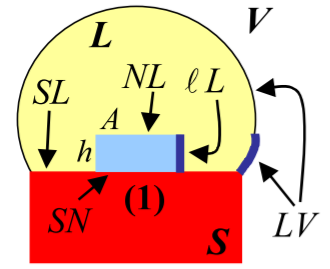
\includegraphics[width=0.3\linewidth]{Image_7_1}}
			\subcaptionbox{\label{fig:Image_7_2}}{%
		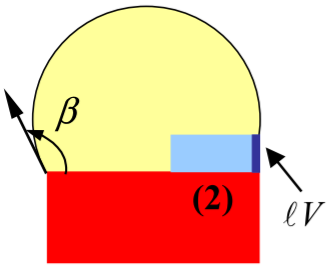
\includegraphics[width=0.3\linewidth]{Image_7_2}} } \legend{Обозначения
	интерфейсов: кристалл\,--\,зародыш \((SN)\), зародыш\,--\,жидкость \((NL)\),
кристалл\,--\,жидкость \((SL)\), жидкость\,--\,пар \((LV)\),
кристалл\,--\,жидкость \((lL)\) и жидкость\,--\,пар \((LV)\); \(\beta\)~---
контактный угол капли} \caption{Схема зарождения вдали от тройной линии~(а) и
на тройной линии~(б) \cite{Glas2007}}\label{fig:Image_7} \end{figure}

В ходе стационарного роста самокаталитических ННК (контактный угол капли
\(\beta\approx 130\){\textdegree}) зарождение происходит вдали от тройной
линии, что приводит к преимущественному формированию структуры ZB
\cite{Cirlin2010}. Для ННК, капли которых израсходованы, характерно наличие в
верхней части последовательность ZB\,--\,WZ\,--\,ZB \cite{Spirkoska2009,
Ambrosini2011}. Это связывают с изменением контактного угла капли от \(\approx
110\){\textdegree} до 0{\textdegree} через значение 90{\textdegree}, где
\(\sin(\beta)\) имеет максимум.

\subsection{Капельная эпитаксия}\label{subsec:ch1/sec2/sub6}

Капельная эпитаксия~--- метод формирования эпитаксиальных наночастиц путем
кристаллизации металлических капель элемента III группы в потоке элемента V
группы (см.~рис.~\cref{fig:Image_8_1}).

\begin{figure}[ht] \centerfloat{ \subcaptionbox{\label{fig:Image_8_1_1}}{%
			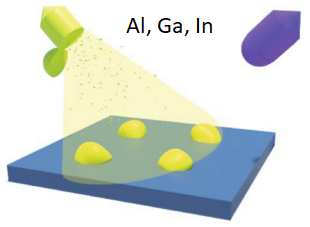
\includegraphics[width=0.3\linewidth]{Image_8_1_1}}
			\subcaptionbox{\label{fig:Image_8_1_2}}{%
		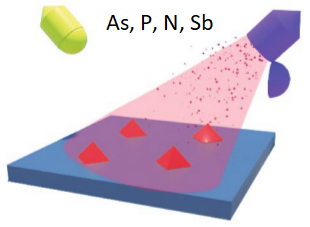
\includegraphics[width=0.3\linewidth]{Image_8_1_2}} } \caption{Схема метода
	капельной эпитаксии: нанесение материала III группы~(а), кристаллизации
капель в потоке элементов V группы~(б) \cite{Gurioli2019}}\label{fig:Image_8_1}
\end{figure}

Нанесение менее монослоя металла на поверхность Si формирует смачивающий слой с
соответствующей реконструкцией (подробнее
см.~подраздел~\cref{subsec:ch2/sec1/sub2}) \cite{Park1988}. Нанесение Ga сверх
монослоя формирует массив капель, плотность и размер которых зависят от
диффузионной длины адатомов и количества нанесенного материала
(см.~рис.~\cref{fig:Image_8_2}). После формирования капель источник металла
закрывают, а капли кристаллизуют под потоком элемента V группы.

\begin{figure}[ht] \centerfloat{ \subcaptionbox{\label{fig:Image_8_2_1}}{%
			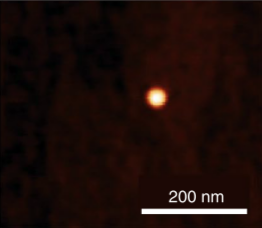
\includegraphics[width=0.3\linewidth]{Image_8_2_1}}
			\subcaptionbox{\label{fig:Image_8_2_2}}{%
		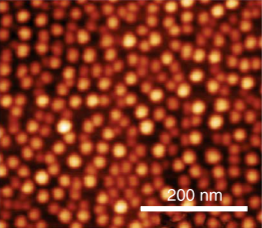
\includegraphics[width=0.3\linewidth]{Image_8_2_2}} } \caption{Пример
	формирования частиц различной плотности при высоких~(а) и низких~(б)
температурах подложки AlGaAs(001) во время осаждения металла
\cite{Gurioli2019}}\label{fig:Image_8_2} \end{figure}

Терминация поверхности элементами V группы вокруг капли может способствовать
миграции адатомов металла из капли. При доминировании этого процесса образуются
кольцеобразные эпитаксиальные частицы (см.~рис.~\cref{fig:Image_8_3})
\cite{Gurioli2019, mano2005}.

\begin{figure}[ht] \centerfloat{ \subcaptionbox{\label{fig:Image_8_3_1}}{%
		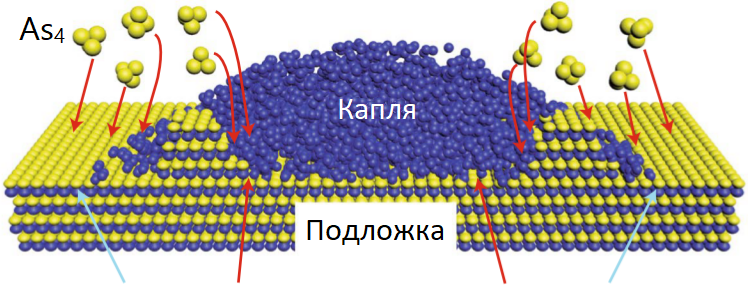
\includegraphics[width=0.65\linewidth]{Image_8_3_1}}

		\subcaptionbox{\label{fig:Image_8_3_2}}{%\textbf{}
	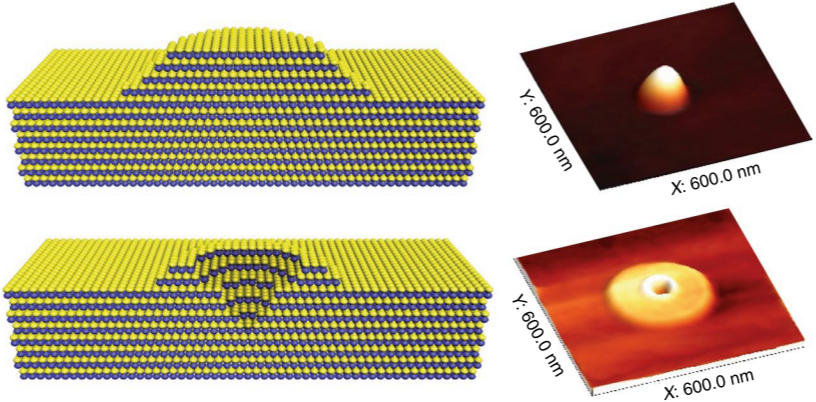
\includegraphics[width=0.65\linewidth]{Image_8_3_2}} } \caption{Схема
процесса капельной эпитаксии~(а). Схема и АСМ изображения островков и
кольцеобразных наноструктур, полученных методом капельной эпитаксии~(б)
\cite{Gurioli2019}}\label{fig:Image_8_3} \end{figure}

\subsection{Бескаталитический механизм роста}\label{subsec:ch1/sec2/sub7}

ННК некоторых материалов (например InAs и III-нитридов) могут быть выращены без
использования капель катализатора по самоиндуцированному механизму
пар\,--\,кристалл \cite{Ristic2008, Bolshakov2014}. Он основан на механизме
островкового роста Вольмера\,--\,Вебера, который реализуется, когда атомы
растущего материала сильнее связаны друг с другом, чем с подложкой.

Синтез таких ННК начинается с образования WZ зародыша с ориентацией [0001]
перпендикулярно ростовой поверхности даже в случае аморфной подложки
\cite{Stoica2008, Corfdir2009}. Ориентация зародыша в плоскости
перпендикулярной направлению роста наследуется от подложки. С увеличением
объема зародыша под влиянием поверхностных энергий адсорбированные атомы
(адатомы) начинают преимущественно встраиваться в плоскость (0001), что
приводит к аксиальному удлинению (см.~рис.~\cref{fig:Image_9})
\cite{Dubrovskii2012b}.

\begin{figure}[ht] \centerfloat{ 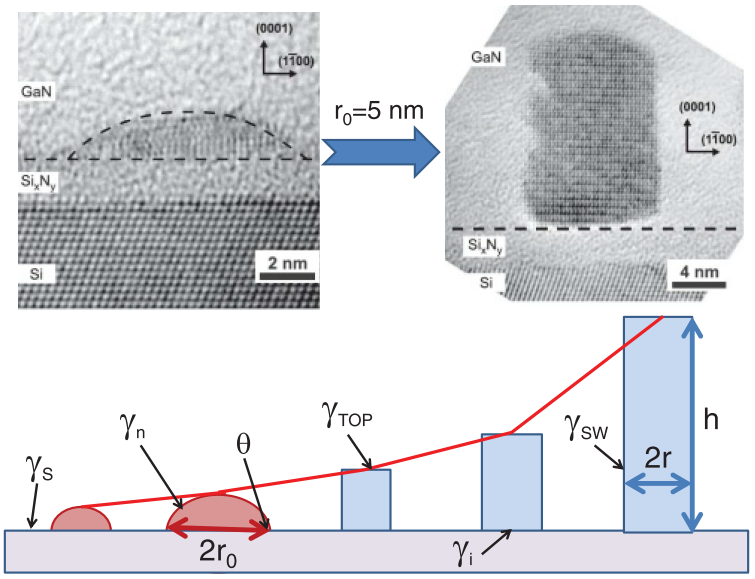
\includegraphics[width=0.7\linewidth]{Image_9}
} \caption{Схема самоиндуцированного механизма роста GaN ННК
\cite{Dubrovskii2012b}}\label{fig:Image_9} \end{figure}

\FloatBarrier
